\documentclass[12pt,letterpaper]{article}\usepackage[]{graphicx}\usepackage[]{color}
%% maxwidth is the original width if it is less than linewidth
%% otherwise use linewidth (to make sure the graphics do not exceed the margin)
\makeatletter
\def\maxwidth{ %
  \ifdim\Gin@nat@width>\linewidth
    \linewidth
  \else
    \Gin@nat@width
  \fi
}
\makeatother

\definecolor{fgcolor}{rgb}{0.345, 0.345, 0.345}
\newcommand{\hlnum}[1]{\textcolor[rgb]{0.686,0.059,0.569}{#1}}%
\newcommand{\hlstr}[1]{\textcolor[rgb]{0.192,0.494,0.8}{#1}}%
\newcommand{\hlcom}[1]{\textcolor[rgb]{0.678,0.584,0.686}{\textit{#1}}}%
\newcommand{\hlopt}[1]{\textcolor[rgb]{0,0,0}{#1}}%
\newcommand{\hlstd}[1]{\textcolor[rgb]{0.345,0.345,0.345}{#1}}%
\newcommand{\hlkwa}[1]{\textcolor[rgb]{0.161,0.373,0.58}{\textbf{#1}}}%
\newcommand{\hlkwb}[1]{\textcolor[rgb]{0.69,0.353,0.396}{#1}}%
\newcommand{\hlkwc}[1]{\textcolor[rgb]{0.333,0.667,0.333}{#1}}%
\newcommand{\hlkwd}[1]{\textcolor[rgb]{0.737,0.353,0.396}{\textbf{#1}}}%

\usepackage{framed}
\makeatletter
\newenvironment{kframe}{%
 \def\at@end@of@kframe{}%
 \ifinner\ifhmode%
  \def\at@end@of@kframe{\end{minipage}}%
  \begin{minipage}{\columnwidth}%
 \fi\fi%
 \def\FrameCommand##1{\hskip\@totalleftmargin \hskip-\fboxsep
 \colorbox{shadecolor}{##1}\hskip-\fboxsep
     % There is no \\@totalrightmargin, so:
     \hskip-\linewidth \hskip-\@totalleftmargin \hskip\columnwidth}%
 \MakeFramed {\advance\hsize-\width
   \@totalleftmargin\z@ \linewidth\hsize
   \@setminipage}}%
 {\par\unskip\endMakeFramed%
 \at@end@of@kframe}
\makeatother

\definecolor{shadecolor}{rgb}{.97, .97, .97}
\definecolor{messagecolor}{rgb}{0, 0, 0}
\definecolor{warningcolor}{rgb}{1, 0, 1}
\definecolor{errorcolor}{rgb}{1, 0, 0}
\newenvironment{knitrout}{}{} % an empty environment to be redefined in TeX

\usepackage{alltt}
\usepackage[utf8]{inputenc}
\usepackage[margin=.7in]{geometry}
\usepackage{graphicx}
\usepackage{titling}
\usepackage{amsmath}
\usepackage{amsfonts}
\usepackage{amssymb}
\renewcommand{\theenumiv}{\arabic{enumiv}}
\setlength{\droptitle}{-5em}
\author{Maurice Diesendruck\vspace{-2ex}}
\title{StatMod2 - Multinomial Dirichlet - Mixture of Normals\vspace{-1ex}}
\IfFileExists{upquote.sty}{\usepackage{upquote}}{}
\begin{document}
\maketitle

\section{Simulated Test Scores}
\subsection{Generate Data}
The school-wide results appear unimodal and slightly skewed left.
\begin{knitrout}
\definecolor{shadecolor}{rgb}{0.969, 0.969, 0.969}\color{fgcolor}\begin{kframe}
\begin{alltt}
\hlstd{simulate.scores} \hlkwb{<-} \hlkwa{function}\hlstd{() \{}
  \hlstd{y.rem} \hlkwb{<-} \hlkwd{rnorm}\hlstd{(}\hlnum{100}\hlstd{,} \hlnum{55}\hlstd{,} \hlnum{15}\hlstd{)}
  \hlstd{y.avg} \hlkwb{<-} \hlkwd{rnorm}\hlstd{(}\hlnum{400}\hlstd{,} \hlnum{70}\hlstd{,} \hlnum{10}\hlstd{)}
  \hlstd{y.hon} \hlkwb{<-} \hlkwd{rnorm}\hlstd{(}\hlnum{150}\hlstd{,} \hlnum{85}\hlstd{,} \hlnum{5}\hlstd{)}
  \hlstd{school.wide} \hlkwb{<-} \hlkwd{c}\hlstd{(y.rem, y.avg, y.hon)}
  \hlkwd{hist}\hlstd{(school.wide,} \hlkwc{breaks}\hlstd{=}\hlnum{100}\hlstd{)}
  \hlkwd{return} \hlstd{(school.wide)}
\hlstd{\}}
\hlstd{school.wide} \hlkwb{<-} \hlkwd{simulate.scores}\hlstd{()}
\end{alltt}
\end{kframe}
\end{knitrout}
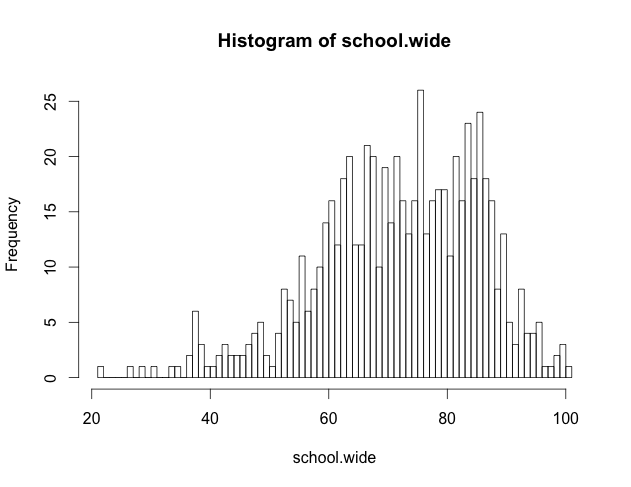
\includegraphics[height=10cm, keepaspectratio]{scores-simulated-data.png}\\

\subsection{Write Full Conditionals}
Write functions to draw from full conditional posterior distributions of
gamma.i and w.
\begin{knitrout}
\definecolor{shadecolor}{rgb}{0.969, 0.969, 0.969}\color{fgcolor}\begin{kframe}
\begin{alltt}
\hlstd{sample.gamma} \hlkwb{<-} \hlkwa{function}\hlstd{(}\hlkwc{y.i}\hlstd{,} \hlkwc{w}\hlstd{) \{}
  \hlkwa{if} \hlstd{(w}\hlopt{==}\hlstd{w1) \{}
    \hlstd{p} \hlkwb{<-} \hlstd{w}\hlopt{*}\hlkwd{dnorm}\hlstd{(y.i,} \hlnum{55}\hlstd{,} \hlnum{15}\hlstd{)}
  \hlstd{\}} \hlkwa{else if} \hlstd{(w}\hlopt{==}\hlstd{w2) \{}
    \hlstd{p} \hlkwb{<-} \hlstd{w}\hlopt{*}\hlkwd{dnorm}\hlstd{(y.i,} \hlnum{70}\hlstd{,} \hlnum{10}\hlstd{)}
  \hlstd{\}} \hlkwa{else if} \hlstd{(w}\hlopt{==}\hlstd{w3) \{}
    \hlstd{p} \hlkwb{<-} \hlstd{w}\hlopt{*}\hlkwd{dnorm}\hlstd{(y.i,} \hlnum{85}\hlstd{,} \hlnum{5}\hlstd{)}
  \hlstd{\}}
  \hlkwd{return} \hlstd{(p)}
\hlstd{\}}
\hlstd{sample.w} \hlkwb{<-} \hlkwa{function}\hlstd{(}\hlkwc{group.counts}\hlstd{=}\hlkwd{c}\hlstd{(n1, n2, n3),} \hlkwc{dir.params}\hlstd{=}\hlkwd{c}\hlstd{(a1, a2, a3)) \{}
  \hlkwd{rdirichlet}\hlstd{(}\hlnum{1}\hlstd{,} \hlkwd{c}\hlstd{(group.counts[}\hlnum{1}\hlstd{]}\hlopt{+}\hlstd{dir.params[}\hlnum{1}\hlstd{],}
                  \hlstd{group.counts[}\hlnum{2}\hlstd{]}\hlopt{+}\hlstd{dir.params[}\hlnum{2}\hlstd{],}
                  \hlstd{group.counts[}\hlnum{3}\hlstd{]}\hlopt{+}\hlstd{dir.params[}\hlnum{3}\hlstd{]))}
\hlstd{\}}
\end{alltt}
\end{kframe}
\end{knitrout}

\subsection{Posterior Given Unknown Mean and Variance}
For a known group $k$, but unknown mean and variance (use sensible priors),
write posterior distribution.\\ 
See page 4 of handwritten notes.\\

\subsection{Gibbs Sampler Results}
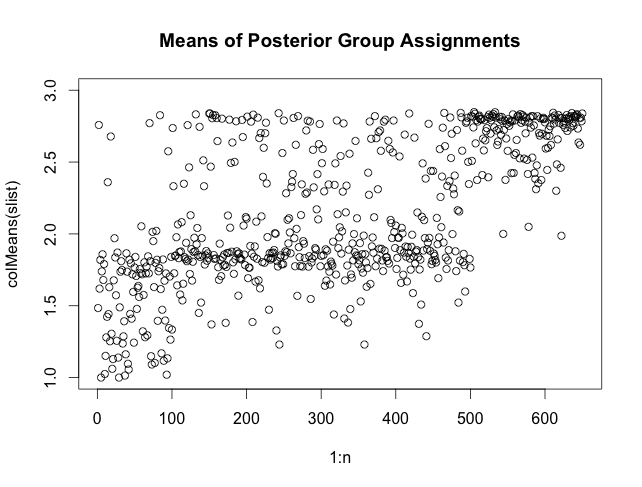
\includegraphics[height=10cm]{scores-posterior-group-assignments.png}\\
\newpage
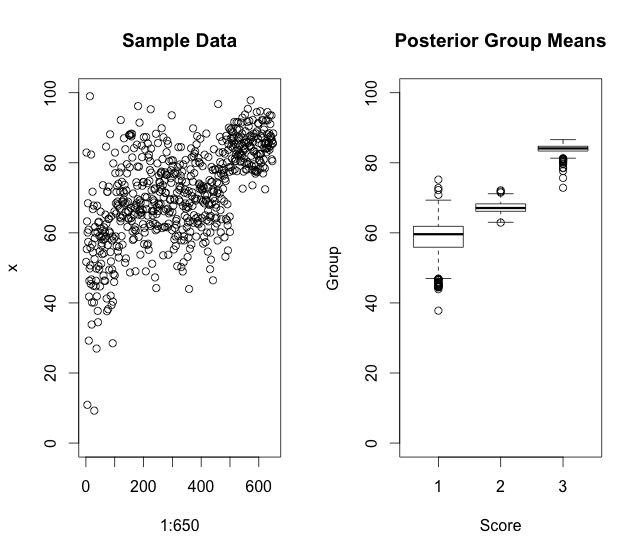
\includegraphics[height=14cm]{scores-sampledata-posteriormeans.png}\\
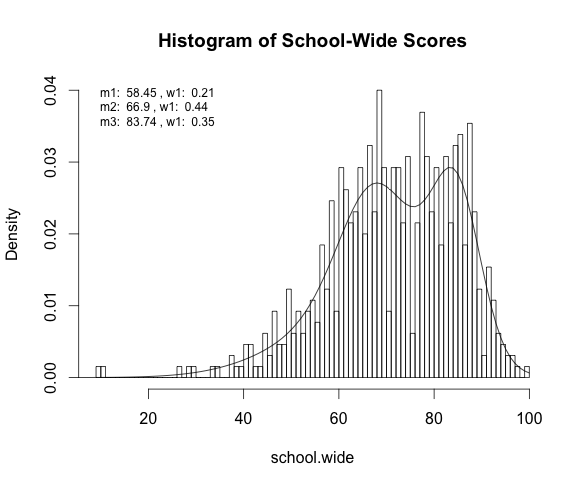
\includegraphics[height=10cm, keepaspectratio]{scores-fitted-mixtures.png}\\


\section{Galaxy Data Set}
Run similar analysis on galaxy data set, with $J=6$.

\subsection{Gibbs Sampler Results}
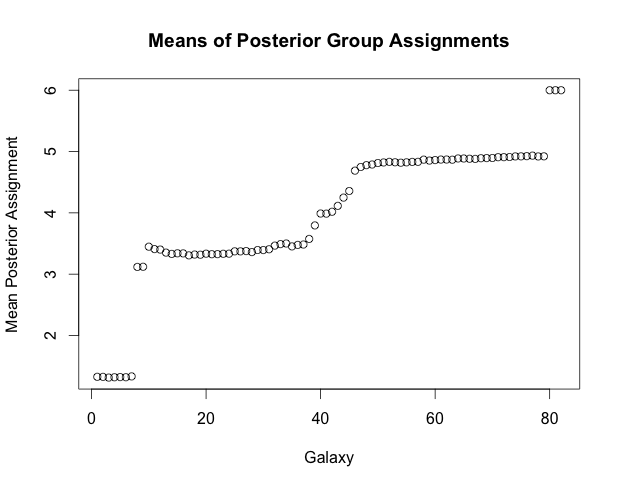
\includegraphics[height=8cm]{gala-posterior-group-assignments.png}\\
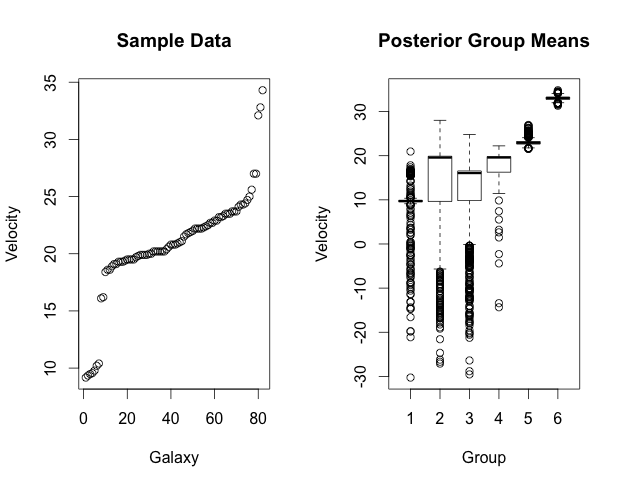
\includegraphics[height=10cm]{gala-sampledata-posteriormeans.png}\\
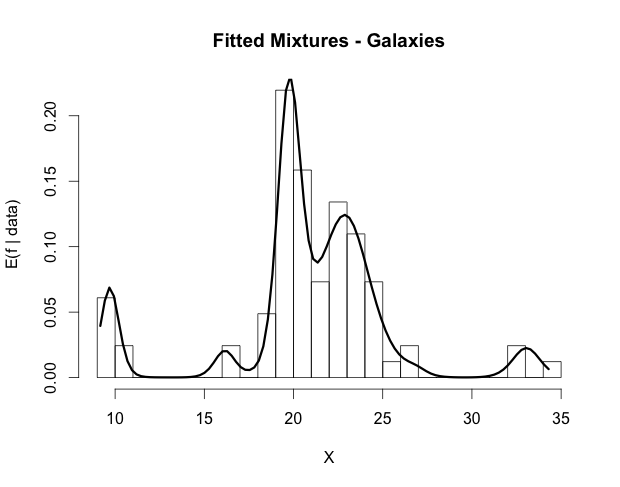
\includegraphics[height=10cm, keepaspectratio]{gala-fitted-mixtures.png}\\

\section{Full R Code}
\begin{knitrout}
\definecolor{shadecolor}{rgb}{0.969, 0.969, 0.969}\color{fgcolor}\begin{kframe}
\begin{alltt}
\hlcom{# Gibbs Sampler}
\hlkwd{require}\hlstd{(}\hlstr{"gtools"}\hlstd{)} \hlcom{## for generating from a Dirichlet distribution}
\hlkwd{require}\hlstd{(}\hlstr{"coda"}\hlstd{)} \hlcom{## for convergence diagonstics}
\hlcom{#x <- scan("galaxies.dta")}
\hlstd{x} \hlkwb{<-} \hlkwd{as.matrix}\hlstd{(}\hlkwd{read.csv}\hlstd{(}\hlstr{"galaxies.csv"} \hlstd{,}\hlkwc{header}\hlstd{=F))}
\hlstd{n} \hlkwb{<-} \hlkwd{length}\hlstd{(x)}
\hlstd{J} \hlkwb{<-} \hlnum{6}
\hlstd{xgrid} \hlkwb{<-} \hlkwd{seq}\hlstd{(}\hlkwc{from}\hlstd{=}\hlkwd{min}\hlstd{(x),}\hlkwc{to}\hlstd{=}\hlkwd{max}\hlstd{(x),}\hlkwc{length}\hlstd{=}\hlnum{100}\hlstd{)}
\hlcom{## hyperparameters for Mu.}
\hlstd{m0} \hlkwb{<-} \hlnum{20}
\hlstd{v0} \hlkwb{<-} \hlnum{100}
\hlcom{## hyperparameters for (1/sig2).}
\hlcom{# 1/sig2 ~ Ga(4, 1) s.t. E(1/sig2) = 4... By guessing that sig=0.5; sig2=0.25;}
\hlcom{# a/b = 1/0.25 = 4/1.}
\hlstd{a0} \hlkwb{<-} \hlnum{4}
\hlstd{b0} \hlkwb{<-} \hlnum{1}
\hlcom{## hyperparameters for dirichlet weights.}
\hlstd{alpha} \hlkwb{<-} \hlnum{1}

\hlstd{sample.s} \hlkwb{<-} \hlkwa{function}\hlstd{(}\hlkwc{w}\hlstd{,} \hlkwc{mu}\hlstd{,} \hlkwc{sig2}\hlstd{) \{}
  \hlcom{## sample s[i] from p(s[i] | ...) }
  \hlstd{n} \hlkwb{<-} \hlkwd{length}\hlstd{(x)}
  \hlstd{sd} \hlkwb{<-} \hlkwd{sqrt}\hlstd{(sig2)}
  \hlstd{s} \hlkwb{<-} \hlkwd{rep}\hlstd{(}\hlnum{0}\hlstd{,n)} \hlcom{# initialize }
  \hlkwa{for}\hlstd{(i} \hlkwa{in} \hlnum{1}\hlopt{:}\hlstd{n)\{}
    \hlstd{pr} \hlkwb{<-} \hlstd{w}\hlopt{*}\hlkwd{dnorm}\hlstd{(x[i],} \hlkwc{m}\hlstd{=mu,} \hlkwc{sd}\hlstd{=sd)}
    \hlstd{s[i]} \hlkwb{<-} \hlkwd{sample}\hlstd{(}\hlnum{1}\hlopt{:}\hlstd{J,} \hlnum{1}\hlstd{,} \hlkwc{replace}\hlstd{=T,} \hlkwc{prob}\hlstd{=pr)}
  \hlstd{\}}
  \hlkwd{return}\hlstd{(s)}
\hlstd{\}}

\hlstd{sample.mu} \hlkwb{<-} \hlkwa{function}\hlstd{(}\hlkwc{s}\hlstd{,} \hlkwc{w}\hlstd{,} \hlkwc{sig2}\hlstd{) \{}
  \hlcom{## sample mu[j] }
  \hlstd{mu} \hlkwb{<-} \hlkwd{rep}\hlstd{(}\hlnum{0}\hlstd{, J)} \hlcom{# initialize }
  \hlkwa{for} \hlstd{(j} \hlkwa{in} \hlnum{1}\hlopt{:}\hlstd{J) \{}
    \hlstd{Aj} \hlkwb{<-} \hlkwd{which}\hlstd{(s}\hlopt{==}\hlstd{j)} \hlcom{# makes vector of indices}
    \hlstd{nj} \hlkwb{<-} \hlkwd{length}\hlstd{(Aj)}
    \hlstd{sig2.j} \hlkwb{<-} \hlstd{sig2[j]}
    \hlkwa{if} \hlstd{(nj}\hlopt{==}\hlnum{0}\hlstd{) \{}
      \hlstd{m} \hlkwb{<-} \hlnum{0}\hlstd{; V} \hlkwb{<-} \hlstd{v0;}
    \hlstd{\}} \hlkwa{else} \hlstd{\{}
      \hlstd{xbar} \hlkwb{<-} \hlkwd{mean}\hlstd{(x[Aj])}
      \hlstd{V} \hlkwb{<-} \hlnum{1}\hlopt{/}\hlstd{(}\hlnum{1}\hlopt{/}\hlstd{v0} \hlopt{+} \hlstd{nj}\hlopt{/}\hlstd{sig2.j)}
      \hlstd{m} \hlkwb{<-} \hlstd{V}\hlopt{*}\hlstd{(m0}\hlopt{/}\hlstd{v0} \hlopt{+} \hlstd{xbar}\hlopt{*}\hlstd{nj}\hlopt{/}\hlstd{sig2.j)}
    \hlstd{\}}
    \hlstd{mu[j]} \hlkwb{<-} \hlkwd{rnorm}\hlstd{(}\hlnum{1}\hlstd{,} \hlkwc{m}\hlstd{=m,} \hlkwc{sd}\hlstd{=}\hlkwd{sqrt}\hlstd{(V))}
  \hlstd{\}}
  \hlkwd{return}\hlstd{(mu)}
\hlstd{\}}

\hlstd{sample.w} \hlkwb{<-} \hlkwa{function}\hlstd{(}\hlkwc{s}\hlstd{) \{}
  \hlcom{## sample w }
  \hlstd{a} \hlkwb{<-} \hlkwd{rep}\hlstd{(}\hlnum{0}\hlstd{,J)} \hlcom{# initialize }
  \hlkwa{for}\hlstd{(j} \hlkwa{in} \hlnum{1}\hlopt{:}\hlstd{J) \{}
    \hlstd{Aj} \hlkwb{<-} \hlkwd{which}\hlstd{(s}\hlopt{==}\hlstd{j)}
    \hlstd{nj} \hlkwb{<-} \hlkwd{length}\hlstd{(Aj)}
    \hlstd{a[j]} \hlkwb{<-} \hlstd{alpha}\hlopt{+}\hlstd{nj}
  \hlstd{\}}
  \hlstd{w} \hlkwb{<-} \hlkwd{rdirichlet}\hlstd{(}\hlnum{1}\hlstd{, a)}
  \hlstd{w} \hlkwb{<-} \hlkwd{c}\hlstd{(w)}
  \hlkwd{return}\hlstd{(w)}
\hlstd{\}}

\hlstd{sample.sig} \hlkwb{<-} \hlkwa{function}\hlstd{(}\hlkwc{s}\hlstd{,} \hlkwc{mu}\hlstd{) \{}
  \hlcom{## sample sig2}
  \hlstd{sig2} \hlkwb{<-} \hlkwd{rep}\hlstd{(}\hlnum{0}\hlstd{, J)}
  \hlkwa{for} \hlstd{(j} \hlkwa{in} \hlnum{1}\hlopt{:}\hlstd{J) \{}
    \hlstd{Aj} \hlkwb{<-} \hlkwd{which}\hlstd{(s}\hlopt{==}\hlstd{j)} \hlcom{# makes vector of indices}
    \hlstd{nj} \hlkwb{<-} \hlkwd{length}\hlstd{(Aj)}
    \hlstd{mu.j} \hlkwb{<-} \hlstd{mu[j]}
    \hlkwa{if} \hlstd{(nj}\hlopt{==}\hlnum{0}\hlstd{) \{}
      \hlstd{a1} \hlkwb{<-} \hlstd{a0; b1} \hlkwb{<-} \hlstd{b0;}
    \hlstd{\}} \hlkwa{else} \hlstd{\{}
      \hlstd{S2} \hlkwb{<-} \hlkwd{sum}\hlstd{((x[Aj]}\hlopt{-}\hlstd{mu.j)}\hlopt{^}\hlnum{2}\hlstd{)}
      \hlstd{a1} \hlkwb{<-} \hlstd{a0} \hlopt{+} \hlstd{nj}\hlopt{/}\hlnum{2}
      \hlstd{b1} \hlkwb{<-} \hlstd{b0} \hlopt{+} \hlstd{S2}\hlopt{/}\hlnum{2}
    \hlstd{\}}
    \hlstd{sig2[j]} \hlkwb{<-} \hlnum{1.0}\hlopt{/}\hlkwd{rgamma}\hlstd{(}\hlnum{1}\hlstd{,} \hlkwc{shape}\hlstd{=a1,} \hlkwc{rate}\hlstd{=b1)}
  \hlstd{\}}
  \hlkwd{return}\hlstd{(sig2)}
\hlstd{\}}

\hlstd{f} \hlkwb{<-} \hlkwa{function}\hlstd{(}\hlkwc{xi}\hlstd{,} \hlkwc{w}\hlstd{,} \hlkwc{mu}\hlstd{,} \hlkwc{sig2}\hlstd{) \{}
  \hlstd{y} \hlkwb{<-} \hlnum{0}
  \hlkwa{for} \hlstd{(j} \hlkwa{in} \hlnum{1}\hlopt{:}\hlstd{J)\{}
    \hlstd{y} \hlkwb{<-} \hlstd{y}\hlopt{+}\hlstd{w[j]}\hlopt{*}\hlkwd{dnorm}\hlstd{(xi,} \hlkwc{m}\hlstd{=mu[j],} \hlkwc{sd}\hlstd{=}\hlkwd{sqrt}\hlstd{(sig2[j]))}
  \hlstd{\}}
  \hlkwd{return}\hlstd{(y)}
\hlstd{\}}

\hlstd{init} \hlkwb{<-} \hlkwa{function}\hlstd{() \{}
  \hlcom{# use some exploratory data analysis for initial values of the parameters}
  \hlcom{# initialize s with a hierarchical tree, cut for J clusters }
  \hlstd{hc} \hlkwb{<-} \hlkwd{hclust}\hlstd{(}\hlkwd{dist}\hlstd{(x),} \hlstr{"ave"}\hlstd{)}
  \hlstd{s} \hlkwb{<-} \hlkwd{cutree}\hlstd{(hc,}\hlkwc{k}\hlstd{=J)}
  \hlstd{mu} \hlkwb{<-} \hlkwd{rnorm}\hlstd{(J,} \hlkwc{m}\hlstd{=m0,} \hlkwc{sd}\hlstd{=}\hlkwd{sqrt}\hlstd{(v0))}
  \hlstd{sig2} \hlkwb{<-} \hlnum{1}\hlopt{/}\hlkwd{rgamma}\hlstd{(J, a0, b0)}
  \hlstd{w} \hlkwb{<-} \hlkwd{rdirichlet}\hlstd{(}\hlnum{1}\hlstd{,} \hlkwd{rep}\hlstd{(alpha, J))}

  \hlkwd{return}\hlstd{(}\hlkwc{th}\hlstd{=}\hlkwd{list}\hlstd{(}\hlkwc{mu}\hlstd{=mu,} \hlkwc{sig2}\hlstd{=sig2,} \hlkwc{w}\hlstd{=w,} \hlkwc{s}\hlstd{=s))}
\hlstd{\}}

\hlstd{gibbs} \hlkwb{<-} \hlkwa{function}\hlstd{(}\hlkwc{n.iter}\hlstd{=}\hlnum{1000}\hlstd{) \{}
  \hlcom{## initialize the parameters }
  \hlstd{th} \hlkwb{<-} \hlkwd{init}\hlstd{()}
  \hlstd{s} \hlkwb{<-} \hlstd{th}\hlopt{$}\hlstd{s; mu} \hlkwb{<-} \hlstd{th}\hlopt{$}\hlstd{mu; sig2} \hlkwb{<-} \hlstd{th}\hlopt{$}\hlstd{sig2; w} \hlkwb{<-} \hlstd{th}\hlopt{$}\hlstd{w}
  \hlcom{## set up lists to save simulations }
  \hlstd{slist} \hlkwb{<-} \hlkwa{NULL}
  \hlstd{mlist} \hlkwb{<-} \hlkwa{NULL}
  \hlstd{flist} \hlkwb{<-} \hlkwa{NULL}
  \hlstd{siglist} \hlkwb{<-} \hlkwa{NULL}
  \hlstd{wlist} \hlkwb{<-} \hlkwa{NULL}

  \hlkwa{for}\hlstd{(iter} \hlkwa{in} \hlnum{1}\hlopt{:}\hlstd{n.iter)\{}
    \hlstd{s} \hlkwb{<-} \hlkwd{sample.s}\hlstd{(w, mu, sig2)}
    \hlstd{mu} \hlkwb{<-} \hlkwd{sample.mu}\hlstd{(s, w, sig2)}
    \hlstd{w} \hlkwb{<-} \hlkwd{sample.w}\hlstd{(s)}
    \hlstd{sig2} \hlkwb{<-} \hlkwd{sample.sig}\hlstd{(s, mu)}
    \hlcom{## save summaries of current simulation }
    \hlstd{slist} \hlkwb{<-} \hlkwd{rbind}\hlstd{(slist, s)}
    \hlstd{mlist} \hlkwb{<-} \hlkwd{rbind}\hlstd{(mlist, mu)}
    \hlstd{siglist} \hlkwb{<-} \hlkwd{c}\hlstd{(siglist, sig2)}
    \hlstd{wlist} \hlkwb{<-} \hlkwd{rbind}\hlstd{(wlist,w)}
    \hlstd{flist} \hlkwb{<-} \hlkwd{rbind}\hlstd{(flist,} \hlkwd{f}\hlstd{(xgrid, w, mu, sig2))}
  \hlstd{\}}
  \hlkwd{return}\hlstd{(}\hlkwd{list}\hlstd{(}\hlkwc{s}\hlstd{=slist,} \hlkwc{m}\hlstd{=mlist,} \hlkwc{f}\hlstd{=flist,} \hlkwc{sig}\hlstd{=siglist,} \hlkwc{w}\hlstd{=wlist))}
\hlstd{\}}

\hlcom{# GET RESULTS}
\hlkwd{dev.off}\hlstd{()}
\hlstd{results} \hlkwb{<-} \hlkwd{gibbs}\hlstd{(}\hlkwc{n.iter}\hlstd{=}\hlnum{2000}\hlstd{)}
\hlstd{slist} \hlkwb{<-} \hlstd{results}\hlopt{$}\hlstd{s}
\hlstd{mlist} \hlkwb{<-} \hlstd{results}\hlopt{$}\hlstd{m}
\hlstd{flist} \hlkwb{<-} \hlstd{results}\hlopt{$}\hlstd{f}
\hlstd{siglist} \hlkwb{<-} \hlstd{results}\hlopt{$}\hlstd{sig}
\hlstd{wlist} \hlkwb{<-} \hlstd{results}\hlopt{$}\hlstd{w}

\hlcom{# Fitted Mixtures Plot}
\hlstd{plt.f} \hlkwb{<-} \hlkwa{function}\hlstd{(}\hlkwc{flist}\hlstd{,} \hlkwc{col}\hlstd{=}\hlnum{1}\hlstd{,} \hlkwc{lty}\hlstd{=}\hlnum{1}\hlstd{,} \hlkwc{add}\hlstd{=F) \{}
  \hlstd{fbar} \hlkwb{<-} \hlkwd{apply}\hlstd{(flist,}\hlnum{2}\hlstd{,mean)}
  \hlkwa{if} \hlstd{(}\hlopt{!}\hlstd{add) \{}
    \hlkwd{hist}\hlstd{(x,} \hlkwc{bty}\hlstd{=}\hlstr{"l"}\hlstd{,} \hlkwc{xlab}\hlstd{=}\hlstr{"X"}\hlstd{,} \hlkwc{ylab}\hlstd{=}\hlstr{"E(f | data)"}\hlstd{,}
         \hlkwc{main}\hlstd{=}\hlstr{"Fitted Mixtures - Galaxies"}\hlstd{,} \hlkwc{prob}\hlstd{=T,}
         \hlkwc{breaks}\hlstd{=}\hlnum{30}\hlstd{)}
  \hlstd{\}}
  \hlkwd{lines}\hlstd{(xgrid, fbar,} \hlkwc{type}\hlstd{=}\hlstr{"l"}\hlstd{,} \hlkwc{lwd}\hlstd{=}\hlnum{3}\hlstd{,} \hlkwc{col}\hlstd{=col,} \hlkwc{lty}\hlstd{=lty)}
\hlstd{\}}
\hlkwd{plt.f}\hlstd{(flist)}

\hlcom{# PLOT RESULTS}
\hlkwd{plot}\hlstd{(}\hlnum{1}\hlopt{:}\hlstd{n,} \hlkwd{colMeans}\hlstd{(slist),} \hlkwc{main}\hlstd{=}\hlstr{"Means of Posterior Group Assignments"}\hlstd{,}
     \hlkwc{xlab}\hlstd{=}\hlstr{"Galaxy"}\hlstd{,} \hlkwc{ylab}\hlstd{=}\hlstr{"Mean Posterior Assignment"}\hlstd{)}
\hlkwd{par}\hlstd{(}\hlkwc{mfrow}\hlstd{=}\hlkwd{c}\hlstd{(}\hlnum{1}\hlstd{,}\hlnum{2}\hlstd{))}
\hlkwd{plot}\hlstd{(}\hlnum{1}\hlopt{:}\hlkwd{length}\hlstd{(x), x,} \hlkwc{main}\hlstd{=}\hlstr{"Sample Data"}\hlstd{,}
     \hlkwc{xlab}\hlstd{=}\hlstr{"Galaxy"}\hlstd{,} \hlkwc{ylab}\hlstd{=}\hlstr{"Velocity"}\hlstd{)}
\hlstd{o} \hlkwb{<-} \hlkwd{order}\hlstd{(}\hlkwd{colMeans}\hlstd{(mlist))}
\hlkwd{boxplot}\hlstd{(}\hlkwd{tail}\hlstd{(mlist[,o],}\hlnum{1000}\hlstd{),} \hlkwc{main}\hlstd{=}\hlstr{"Posterior Group Means"}\hlstd{,}
        \hlkwc{xlab}\hlstd{=}\hlstr{"Group"}\hlstd{,} \hlkwc{ylab}\hlstd{=}\hlstr{"Velocity"}\hlstd{)}
\end{alltt}
\end{kframe}
\end{knitrout}
\end{document}


